\chapter{Hosted AST Interpreter}

Abstract syntax trees, ASTs, are the simplest and most natural ways to implement programming languages.
They do not require an additional translation step that linearizes ASTs produced by the parser to bytecode or other forms of internal representations.
They also lend themselves well to optimizations that are particularly beneficial to highly dynamic languages like Python.

We present ZipPy, a Python 3 implementation that is hosted on the JVM.
ZipPy incorporates recent works on self-optimizing AST interpreters for the JVM.
Our work however focuses on high level guest language features that are distinct in Python and
how well we can fit them onto the existing optimizing AST interpreter framework.

\section{Python on Truffle}

\begin{figure}[t]
\centering
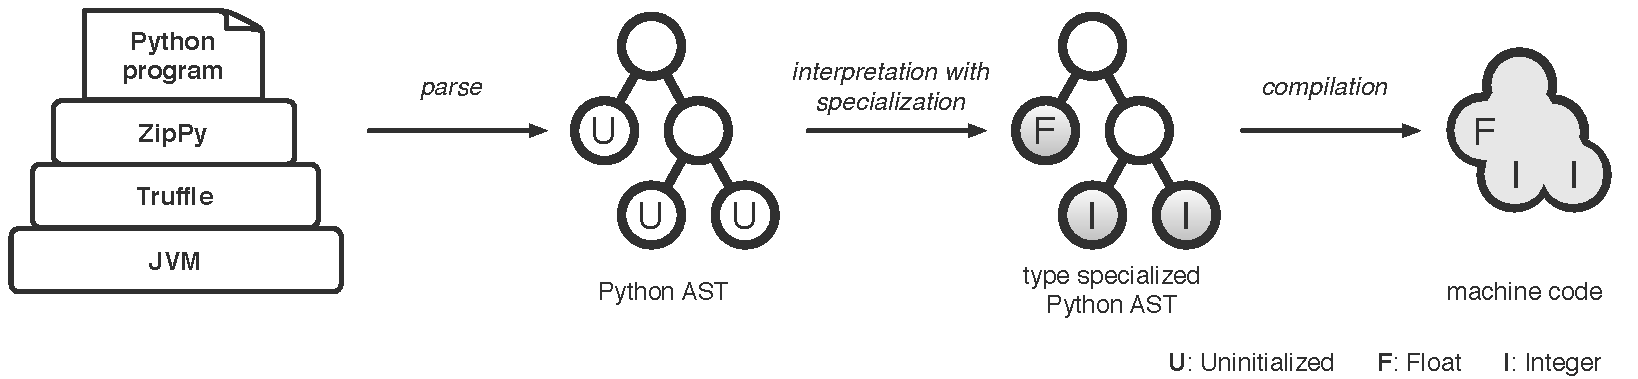
\includegraphics[scale=.6]{figures/ch3-python-on-truffle.pdf}
\caption{Python on Truffle}
\label{fig:python-on-truffle}
\end{figure}

In principle, ``everything'' can change at any moment in dynamic language programs.
This dynamic nature is the major impediment to ahead-of-time optimization.
In practice, however, programmers tend to minimize the rate of change, which makes the code highly predictable.
Types, for instance, typically remain stable between successive executions of a particular operation instance.
Deutsch and Schiffman report that speculative type specialization succeeds $95\%$ of the time in their classic Smalltalk-80 implementation~\cite{Deutsch1984}.

Truffle is a self-optimizing runtime system that makes it easy to perform type specialization for dynamic languages running on top of the JVM~\cite{Wurthinger+13}.
It allows language implementers to implement their guest language by writing an AST interpreter using Java.
An interpreter written in this way enjoys low cost type specialization via automatic node rewriting~\cite{Wurthinger+12,Brunthaler2010inca,Brunthaler2010quickening}.
AST node rewriting collects runtime type information, and speculatively replaces the existing nodes with specialized and more efficient ones.
Subsequently, Truffle just-in-time compiles the specialized AST, written in Java, directly to machine code using the underlying Java compiler.
Upon a type mis-speculation, the specialized AST node handles the type change by replacing itself with a more generic one.
The node replacement triggers deoptimization from the compiled code and transfers execution back to the interpreter.
If the re-specialized AST stays stable, Truffle can again compile it to machine code.

Our system, ZipPy, is a full-fledged prototype Python 3 implementation built atop Truffle.
It leverages Truffle's type specialization feature and its underlying compilation infrastructure (see Figure~\ref{fig:python-on-truffle}).
This architecture helps ZipPy outperform Python implementations that either do not exploit runtime type specialization or lack a just-in-time compiler.
However, Truffle has no knowledge about specific high level guest language semantics, like generators in Python.
Further performance exploration of a guest language will mainly benefit from better insights on distinct features of the language and
making better use of the host compiler based on those insights.
In this thesis we focus on guest language level optimizations we added to ZipPy.

\section{Design and Implementation}

ZipPy benefits from the Truffle framework in two ways.
First, Truffle's Java annotation based domain specific language (DSL) greatly simplifies the implementation of type specialization in dynamic languages like Python~\cite{Humer+2014}.
Second, Truffle bridges the gap between the hosted AST interpreter and the underlying Java JIT compiler.
It empowers the hosted interpreter with the performance of a custom compiler without having the hosted VM implementers to actually write a compiler.
The end performance one could achieve on Truffle usually surpasses that of a custom build class file compiler not to mention the upfront cost of building such compiler.

However, Truffle is not a fool proof framework.
It does require knowledge of the Java compiler internals to make better use of the framework.
In this section we describe design choices we made to retrofit the core part of the Python language onto Truffle's execution model.

\subsection{Applying Type Specialization}

\begin{figure}[t]
\centering
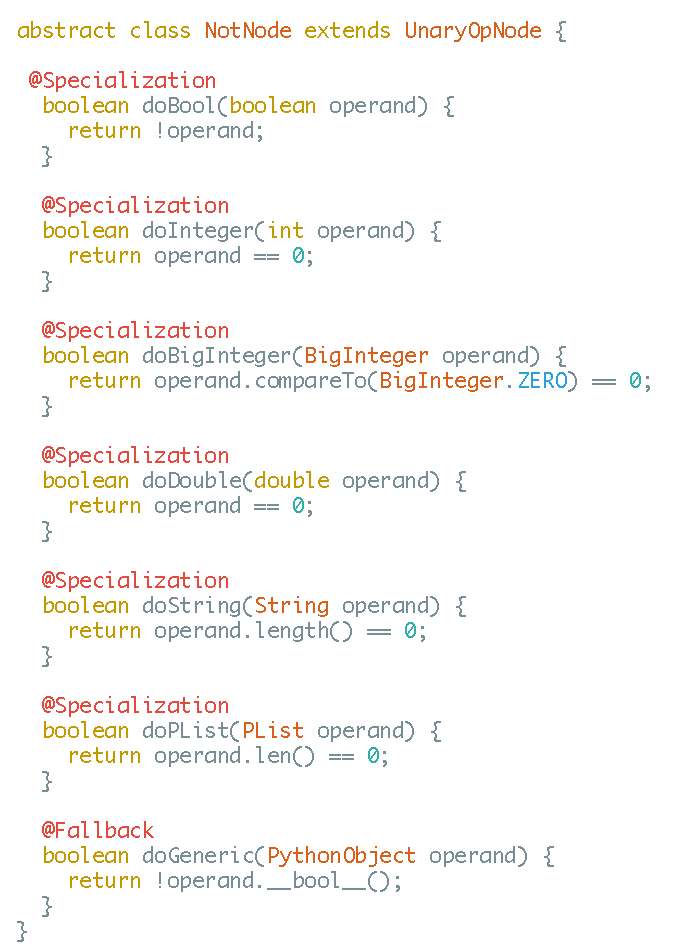
\includegraphics[scale=1]{figures/ch3-not-node.pdf}
\caption{Implementation of \texttt{NotNode} in ZipPy}
\label{fig:not-node}
\end{figure}

\subsection{Numeric Types}

\subsection{Comnposite Data Types}
